\begin{figure}[H]
\centering
\begin{minipage}[t]{0.48\textwidth}
\centering

  \begin{tikzpicture}[scale=0.8]
    \fill[gray] (0, 0) rectangle (1, 1);
    \fill[gray] (2, 0) rectangle (3, 1);
    \fill[gray] (4, 0) rectangle (5, 1);
    \fill[gray] (0, 1) rectangle (1, 2);
    \fill[gray] (2, 1) rectangle (3, 2);
    \node at (0.5, 2.5){\color{blue}\faIcon{user}};
    \fill[gray] (4, 2) rectangle (5, 3);
    \fill[gray] (2, 3) rectangle (3, 4);
    \fill[gray] (4, 3) rectangle (5, 4);
    \fill[gray] (0, 4) rectangle (1, 5);
    \fill[gray] (2, 4) rectangle (3, 5);
    \node at (3.5, 4.5){\color{blue}\faIcon{home}};
    \fill[gray] (4, 4) rectangle (5, 5);
    \draw[black] grid (5, 5);
  \end{tikzpicture}

  \caption{\centering Dodaj do kolejki węzeł (0,2).}
  \label{fig:bfs_solve_steps_start}
\end{minipage}\hfill
\begin{minipage}[t]{0.48\textwidth}
  \centering

  \begin{tikzpicture}[scale=0.8]
    \fill[gray] (0, 0) rectangle (1, 1);
    \fill[gray] (2, 0) rectangle (3, 1);
    \fill[gray] (4, 0) rectangle (5, 1);
    \fill[gray] (0, 1) rectangle (1, 2);
    \fill[gray] (2, 1) rectangle (3, 2);
    \node at (0.5, 2.5){\color{blue}\faIcon{user}};
    \fill[gray] (4, 2) rectangle (5, 3);
    \fill[gray] (2, 3) rectangle (3, 4);
    \fill[gray] (4, 3) rectangle (5, 4);
    \fill[gray] (0, 4) rectangle (1, 5);
    \fill[gray] (2, 4) rectangle (3, 5);
    \node at (3.5, 4.5){\color{blue}\faIcon{home}};
    \fill[gray] (4, 4) rectangle (5, 5);
    \draw[black] grid (5, 5);
  \end{tikzpicture}

  \caption{\centering Rozpatrz pole pole (0,2).}
\end{minipage}
\end{figure}

\begin{figure}[H]
\centering
\begin{minipage}[t]{0.48\textwidth}
  \centering

  \begin{tikzpicture}[scale=0.8]
    \fill[gray] (0, 0) rectangle (1, 1);
    \fill[gray] (2, 0) rectangle (3, 1);
    \fill[gray] (4, 0) rectangle (5, 1);
    \fill[gray] (0, 1) rectangle (1, 2);
    \fill[gray] (2, 1) rectangle (3, 2);
    \node at (0.5, 2.5){\color{blue}\faIcon{user}};
    \node at (1.5, 2.5){\color{purple}\faIcon{hourglass}};
    \fill[gray] (4, 2) rectangle (5, 3);
    \fill[gray] (2, 3) rectangle (3, 4);
    \fill[gray] (4, 3) rectangle (5, 4);
    \fill[gray] (0, 4) rectangle (1, 5);
    \fill[gray] (2, 4) rectangle (3, 5);
    \node at (3.5, 4.5){\color{blue}\faIcon{home}};
    \fill[gray] (4, 4) rectangle (5, 5);
    \draw[black] grid (5, 5);
  \end{tikzpicture}

  \caption{\centering Dodaj do kolejki węzeł (1,2).}
\end{minipage}\hfill
\begin{minipage}[t]{0.48\textwidth}
  \centering

  \begin{tikzpicture}[scale=0.8]
    \fill[gray] (0, 0) rectangle (1, 1);
    \fill[gray] (2, 0) rectangle (3, 1);
    \fill[gray] (4, 0) rectangle (5, 1);
    \fill[gray] (0, 1) rectangle (1, 2);
    \fill[gray] (2, 1) rectangle (3, 2);
    \node at (0.5, 2.5){\color{blue}\faIcon{user}};
    \node at (1.5, 2.5){\color{purple}\faIcon{hourglass}};
    \fill[gray] (4, 2) rectangle (5, 3);
    \node at (0.5, 3.5){\color{purple}\faIcon{hourglass}};
    \fill[gray] (2, 3) rectangle (3, 4);
    \fill[gray] (4, 3) rectangle (5, 4);
    \fill[gray] (0, 4) rectangle (1, 5);
    \fill[gray] (2, 4) rectangle (3, 5);
    \node at (3.5, 4.5){\color{blue}\faIcon{home}};
    \fill[gray] (4, 4) rectangle (5, 5);
    \draw[black] grid (5, 5);
  \end{tikzpicture}

  \caption{\centering Dodaj do kolejki węzeł (0,3).}
\end{minipage}
\end{figure}

\begin{figure}[H]
\centering
\begin{minipage}[t]{0.48\textwidth}
  \centering

  \begin{tikzpicture}[scale=0.8]
    \fill[gray] (0, 0) rectangle (1, 1);
    \fill[gray] (2, 0) rectangle (3, 1);
    \fill[gray] (4, 0) rectangle (5, 1);
    \fill[gray] (0, 1) rectangle (1, 2);
    \fill[gray] (2, 1) rectangle (3, 2);
    \node at (0.5, 2.5){\color{blue}\faIcon{user}};
    \node at (1.5, 2.5){\color{orange}\faIcon{arrows-alt}};
    \fill[gray] (4, 2) rectangle (5, 3);
    \node at (0.5, 3.5){\color{purple}\faIcon{hourglass}};
    \fill[gray] (2, 3) rectangle (3, 4);
    \fill[gray] (4, 3) rectangle (5, 4);
    \fill[gray] (0, 4) rectangle (1, 5);
    \fill[gray] (2, 4) rectangle (3, 5);
    \node at (3.5, 4.5){\color{blue}\faIcon{home}};
    \fill[gray] (4, 4) rectangle (5, 5);
    \draw[black] grid (5, 5);
  \end{tikzpicture}

  \caption{\centering Rozpatrz pole (1,2).}
\end{minipage}\hfill
\begin{minipage}[t]{0.48\textwidth}
  \centering

  \begin{tikzpicture}[scale=0.8]
    \fill[gray] (0, 0) rectangle (1, 1);
    \fill[gray] (2, 0) rectangle (3, 1);
    \fill[gray] (4, 0) rectangle (5, 1);
    \fill[gray] (0, 1) rectangle (1, 2);
    \fill[gray] (2, 1) rectangle (3, 2);
    \node at (0.5, 2.5){\color{blue}\faIcon{user}};
    \node at (1.5, 2.5){\color{orange}\faIcon{arrows-alt}};
    \fill[gray] (4, 2) rectangle (5, 3);
    \node at (0.5, 3.5){\color{purple}\faIcon{hourglass}};
    \fill[gray] (2, 3) rectangle (3, 4);
    \fill[gray] (4, 3) rectangle (5, 4);
    \fill[gray] (0, 4) rectangle (1, 5);
    \fill[gray] (2, 4) rectangle (3, 5);
    \node at (3.5, 4.5){\color{blue}\faIcon{home}};
    \fill[gray] (4, 4) rectangle (5, 5);
    \draw[black] grid (5, 5);
  \end{tikzpicture}

  \caption{\centering Dodaj do kolejki węzeł (0,2).}
\end{minipage}
\end{figure}

\begin{figure}[H]
\centering
\begin{minipage}[t]{0.48\textwidth}
  \centering

  \begin{tikzpicture}[scale=0.8]
    \fill[gray] (0, 0) rectangle (1, 1);
    \fill[gray] (2, 0) rectangle (3, 1);
    \fill[gray] (4, 0) rectangle (5, 1);
    \fill[gray] (0, 1) rectangle (1, 2);
    \node at (1.5, 1.5){\color{purple}\faIcon{hourglass}};
    \fill[gray] (2, 1) rectangle (3, 2);
    \node at (0.5, 2.5){\color{blue}\faIcon{user}};
    \node at (1.5, 2.5){\color{orange}\faIcon{arrows-alt}};
    \fill[gray] (4, 2) rectangle (5, 3);
    \node at (0.5, 3.5){\color{purple}\faIcon{hourglass}};
    \fill[gray] (2, 3) rectangle (3, 4);
    \fill[gray] (4, 3) rectangle (5, 4);
    \fill[gray] (0, 4) rectangle (1, 5);
    \fill[gray] (2, 4) rectangle (3, 5);
    \node at (3.5, 4.5){\color{blue}\faIcon{home}};
    \fill[gray] (4, 4) rectangle (5, 5);
    \draw[black] grid (5, 5);
  \end{tikzpicture}

  \caption{\centering Dodaj do kolejki węzeł (1,1).}
\end{minipage}\hfill
\begin{minipage}[t]{0.48\textwidth}
  \centering

  \begin{tikzpicture}[scale=0.8]
    \fill[gray] (0, 0) rectangle (1, 1);
    \fill[gray] (2, 0) rectangle (3, 1);
    \fill[gray] (4, 0) rectangle (5, 1);
    \fill[gray] (0, 1) rectangle (1, 2);
    \node at (1.5, 1.5){\color{purple}\faIcon{hourglass}};
    \fill[gray] (2, 1) rectangle (3, 2);
    \node at (0.5, 2.5){\color{blue}\faIcon{user}};
    \node at (1.5, 2.5){\color{orange}\faIcon{arrows-alt}};
    \fill[gray] (4, 2) rectangle (5, 3);
    \node at (0.5, 3.5){\color{purple}\faIcon{hourglass}};
    \node at (1.5, 3.5){\color{purple}\faIcon{hourglass}};
    \fill[gray] (2, 3) rectangle (3, 4);
    \fill[gray] (4, 3) rectangle (5, 4);
    \fill[gray] (0, 4) rectangle (1, 5);
    \fill[gray] (2, 4) rectangle (3, 5);
    \node at (3.5, 4.5){\color{blue}\faIcon{home}};
    \fill[gray] (4, 4) rectangle (5, 5);
    \draw[black] grid (5, 5);
  \end{tikzpicture}

  \caption{\centering Dodaj do kolejki węzeł (1,3).}
\end{minipage}
\end{figure}

\begin{figure}[H]
\centering
\begin{minipage}[t]{0.48\textwidth}
  \centering

  \begin{tikzpicture}[scale=0.8]
    \fill[gray] (0, 0) rectangle (1, 1);
    \fill[gray] (2, 0) rectangle (3, 1);
    \fill[gray] (4, 0) rectangle (5, 1);
    \fill[gray] (0, 1) rectangle (1, 2);
    \node at (1.5, 1.5){\color{purple}\faIcon{hourglass}};
    \fill[gray] (2, 1) rectangle (3, 2);
    \node at (0.5, 2.5){\color{blue}\faIcon{user}};
    \node at (1.5, 2.5){\color{orange}\faIcon{arrows-alt}};
    \node at (2.5, 2.5){\color{purple}\faIcon{hourglass}};
    \fill[gray] (4, 2) rectangle (5, 3);
    \node at (0.5, 3.5){\color{purple}\faIcon{hourglass}};
    \node at (1.5, 3.5){\color{purple}\faIcon{hourglass}};
    \fill[gray] (2, 3) rectangle (3, 4);
    \fill[gray] (4, 3) rectangle (5, 4);
    \fill[gray] (0, 4) rectangle (1, 5);
    \fill[gray] (2, 4) rectangle (3, 5);
    \node at (3.5, 4.5){\color{blue}\faIcon{home}};
    \fill[gray] (4, 4) rectangle (5, 5);
    \draw[black] grid (5, 5);
  \end{tikzpicture}

  \caption{\centering Dodaj do kolejki węzeł (2,2).}
\end{minipage}\hfill
\begin{minipage}[t]{0.48\textwidth}
  \centering

  \begin{tikzpicture}[scale=0.8]
    \fill[gray] (0, 0) rectangle (1, 1);
    \fill[gray] (2, 0) rectangle (3, 1);
    \fill[gray] (4, 0) rectangle (5, 1);
    \fill[gray] (0, 1) rectangle (1, 2);
    \node at (1.5, 1.5){\color{purple}\faIcon{hourglass}};
    \fill[gray] (2, 1) rectangle (3, 2);
    \node at (0.5, 2.5){\color{blue}\faIcon{user}};
    \node at (1.5, 2.5){\color{orange}\faIcon{arrows-alt}};
    \node at (2.5, 2.5){\color{purple}\faIcon{hourglass}};
    \fill[gray] (4, 2) rectangle (5, 3);
    \node at (0.5, 3.5){\color{orange}\faIcon{arrows-alt}};
    \node at (1.5, 3.5){\color{purple}\faIcon{hourglass}};
    \fill[gray] (2, 3) rectangle (3, 4);
    \fill[gray] (4, 3) rectangle (5, 4);
    \fill[gray] (0, 4) rectangle (1, 5);
    \fill[gray] (2, 4) rectangle (3, 5);
    \node at (3.5, 4.5){\color{blue}\faIcon{home}};
    \fill[gray] (4, 4) rectangle (5, 5);
    \draw[black] grid (5, 5);
  \end{tikzpicture}

  \caption{\centering Rozpatrz pole (0,3).}
\end{minipage}
\end{figure}

\begin{figure}[H]
\centering
\begin{minipage}[t]{0.48\textwidth}
  \centering

  \begin{tikzpicture}[scale=0.8]
    \fill[gray] (0, 0) rectangle (1, 1);
    \fill[gray] (2, 0) rectangle (3, 1);
    \fill[gray] (4, 0) rectangle (5, 1);
    \fill[gray] (0, 1) rectangle (1, 2);
    \node at (1.5, 1.5){\color{purple}\faIcon{hourglass}};
    \fill[gray] (2, 1) rectangle (3, 2);
    \node at (0.5, 2.5){\color{blue}\faIcon{user}};
    \node at (1.5, 2.5){\color{orange}\faIcon{arrows-alt}};
    \node at (2.5, 2.5){\color{purple}\faIcon{hourglass}};
    \fill[gray] (4, 2) rectangle (5, 3);
    \node at (0.5, 3.5){\color{orange}\faIcon{arrows-alt}};
    \node at (1.5, 3.5){\color{purple}\faIcon{hourglass}};
    \fill[gray] (2, 3) rectangle (3, 4);
    \fill[gray] (4, 3) rectangle (5, 4);
    \fill[gray] (0, 4) rectangle (1, 5);
    \fill[gray] (2, 4) rectangle (3, 5);
    \node at (3.5, 4.5){\color{blue}\faIcon{home}};
    \fill[gray] (4, 4) rectangle (5, 5);
    \draw[black] grid (5, 5);
  \end{tikzpicture}

  \caption{\centering Rozpatrz pole (0,2).}
\end{minipage}\hfill
\begin{minipage}[t]{0.48\textwidth}
  \centering

  \begin{tikzpicture}[scale=0.8]
    \fill[gray] (0, 0) rectangle (1, 1);
    \fill[gray] (2, 0) rectangle (3, 1);
    \fill[gray] (4, 0) rectangle (5, 1);
    \fill[gray] (0, 1) rectangle (1, 2);
    \node at (1.5, 1.5){\color{orange}\faIcon{arrows-alt}};
    \fill[gray] (2, 1) rectangle (3, 2);
    \node at (0.5, 2.5){\color{blue}\faIcon{user}};
    \node at (1.5, 2.5){\color{orange}\faIcon{arrows-alt}};
    \node at (2.5, 2.5){\color{purple}\faIcon{hourglass}};
    \fill[gray] (4, 2) rectangle (5, 3);
    \node at (0.5, 3.5){\color{orange}\faIcon{arrows-alt}};
    \node at (1.5, 3.5){\color{purple}\faIcon{hourglass}};
    \fill[gray] (2, 3) rectangle (3, 4);
    \fill[gray] (4, 3) rectangle (5, 4);
    \fill[gray] (0, 4) rectangle (1, 5);
    \fill[gray] (2, 4) rectangle (3, 5);
    \node at (3.5, 4.5){\color{blue}\faIcon{home}};
    \fill[gray] (4, 4) rectangle (5, 5);
    \draw[black] grid (5, 5);
  \end{tikzpicture}

  \caption{\centering Rozpatrz pole (1,1).}
\end{minipage}
\end{figure}

\begin{figure}[H]
\centering
\begin{minipage}[t]{0.48\textwidth}
  \centering

  \begin{tikzpicture}[scale=0.8]
    \fill[gray] (0, 0) rectangle (1, 1);
    \node at (1.5, 0.5){\color{purple}\faIcon{hourglass}};
    \fill[gray] (2, 0) rectangle (3, 1);
    \fill[gray] (4, 0) rectangle (5, 1);
    \fill[gray] (0, 1) rectangle (1, 2);
    \node at (1.5, 1.5){\color{orange}\faIcon{arrows-alt}};
    \fill[gray] (2, 1) rectangle (3, 2);
    \node at (0.5, 2.5){\color{blue}\faIcon{user}};
    \node at (1.5, 2.5){\color{orange}\faIcon{arrows-alt}};
    \node at (2.5, 2.5){\color{purple}\faIcon{hourglass}};
    \fill[gray] (4, 2) rectangle (5, 3);
    \node at (0.5, 3.5){\color{orange}\faIcon{arrows-alt}};
    \node at (1.5, 3.5){\color{purple}\faIcon{hourglass}};
    \fill[gray] (2, 3) rectangle (3, 4);
    \fill[gray] (4, 3) rectangle (5, 4);
    \fill[gray] (0, 4) rectangle (1, 5);
    \fill[gray] (2, 4) rectangle (3, 5);
    \node at (3.5, 4.5){\color{blue}\faIcon{home}};
    \fill[gray] (4, 4) rectangle (5, 5);
    \draw[black] grid (5, 5);
  \end{tikzpicture}

  \caption{\centering Dodaj do kolejki węzeł (1,0).}
\end{minipage}\hfill
\begin{minipage}[t]{0.48\textwidth}
  \centering

  \begin{tikzpicture}[scale=0.8]
    \fill[gray] (0, 0) rectangle (1, 1);
    \node at (1.5, 0.5){\color{purple}\faIcon{hourglass}};
    \fill[gray] (2, 0) rectangle (3, 1);
    \fill[gray] (4, 0) rectangle (5, 1);
    \fill[gray] (0, 1) rectangle (1, 2);
    \node at (1.5, 1.5){\color{orange}\faIcon{arrows-alt}};
    \fill[gray] (2, 1) rectangle (3, 2);
    \node at (0.5, 2.5){\color{blue}\faIcon{user}};
    \node at (1.5, 2.5){\color{orange}\faIcon{arrows-alt}};
    \node at (2.5, 2.5){\color{purple}\faIcon{hourglass}};
    \fill[gray] (4, 2) rectangle (5, 3);
    \node at (0.5, 3.5){\color{orange}\faIcon{arrows-alt}};
    \node at (1.5, 3.5){\color{orange}\faIcon{arrows-alt}};
    \fill[gray] (2, 3) rectangle (3, 4);
    \fill[gray] (4, 3) rectangle (5, 4);
    \fill[gray] (0, 4) rectangle (1, 5);
    \fill[gray] (2, 4) rectangle (3, 5);
    \node at (3.5, 4.5){\color{blue}\faIcon{home}};
    \fill[gray] (4, 4) rectangle (5, 5);
    \draw[black] grid (5, 5);
  \end{tikzpicture}

  \caption{\centering Rozpatrz pole (1,3).}
\end{minipage}
\end{figure}

\begin{figure}[H]
\centering
\begin{minipage}[t]{0.48\textwidth}
  \centering

  \begin{tikzpicture}[scale=0.8]
    \fill[gray] (0, 0) rectangle (1, 1);
    \node at (1.5, 0.5){\color{purple}\faIcon{hourglass}};
    \fill[gray] (2, 0) rectangle (3, 1);
    \fill[gray] (4, 0) rectangle (5, 1);
    \fill[gray] (0, 1) rectangle (1, 2);
    \node at (1.5, 1.5){\color{orange}\faIcon{arrows-alt}};
    \fill[gray] (2, 1) rectangle (3, 2);
    \node at (0.5, 2.5){\color{blue}\faIcon{user}};
    \node at (1.5, 2.5){\color{orange}\faIcon{arrows-alt}};
    \node at (2.5, 2.5){\color{purple}\faIcon{hourglass}};
    \fill[gray] (4, 2) rectangle (5, 3);
    \node at (0.5, 3.5){\color{orange}\faIcon{arrows-alt}};
    \node at (1.5, 3.5){\color{orange}\faIcon{arrows-alt}};
    \fill[gray] (2, 3) rectangle (3, 4);
    \fill[gray] (4, 3) rectangle (5, 4);
    \fill[gray] (0, 4) rectangle (1, 5);
    \node at (1.5, 4.5){\color{purple}\faIcon{hourglass}};
    \fill[gray] (2, 4) rectangle (3, 5);
    \node at (3.5, 4.5){\color{blue}\faIcon{home}};
    \fill[gray] (4, 4) rectangle (5, 5);
    \draw[black] grid (5, 5);
  \end{tikzpicture}

  \caption{\centering Dodaj do kolejki węzeł (1,4).}
\end{minipage}\hfill
\begin{minipage}[t]{0.48\textwidth}
  \centering

  \begin{tikzpicture}[scale=0.8]
    \fill[gray] (0, 0) rectangle (1, 1);
    \node at (1.5, 0.5){\color{purple}\faIcon{hourglass}};
    \fill[gray] (2, 0) rectangle (3, 1);
    \fill[gray] (4, 0) rectangle (5, 1);
    \fill[gray] (0, 1) rectangle (1, 2);
    \node at (1.5, 1.5){\color{orange}\faIcon{arrows-alt}};
    \fill[gray] (2, 1) rectangle (3, 2);
    \node at (0.5, 2.5){\color{blue}\faIcon{user}};
    \node at (1.5, 2.5){\color{orange}\faIcon{arrows-alt}};
    \node at (2.5, 2.5){\color{orange}\faIcon{arrows-alt}};
    \fill[gray] (4, 2) rectangle (5, 3);
    \node at (0.5, 3.5){\color{orange}\faIcon{arrows-alt}};
    \node at (1.5, 3.5){\color{orange}\faIcon{arrows-alt}};
    \fill[gray] (2, 3) rectangle (3, 4);
    \fill[gray] (4, 3) rectangle (5, 4);
    \fill[gray] (0, 4) rectangle (1, 5);
    \node at (1.5, 4.5){\color{purple}\faIcon{hourglass}};
    \fill[gray] (2, 4) rectangle (3, 5);
    \node at (3.5, 4.5){\color{blue}\faIcon{home}};
    \fill[gray] (4, 4) rectangle (5, 5);
    \draw[black] grid (5, 5);
  \end{tikzpicture}

  \caption{\centering Rozpatrz pole (2,2).}
\end{minipage}
\end{figure}

\begin{figure}[H]
\centering
\begin{minipage}[t]{0.48\textwidth}
  \centering

  \begin{tikzpicture}[scale=0.8]
    \fill[gray] (0, 0) rectangle (1, 1);
    \node at (1.5, 0.5){\color{purple}\faIcon{hourglass}};
    \fill[gray] (2, 0) rectangle (3, 1);
    \fill[gray] (4, 0) rectangle (5, 1);
    \fill[gray] (0, 1) rectangle (1, 2);
    \node at (1.5, 1.5){\color{orange}\faIcon{arrows-alt}};
    \fill[gray] (2, 1) rectangle (3, 2);
    \node at (0.5, 2.5){\color{blue}\faIcon{user}};
    \node at (1.5, 2.5){\color{orange}\faIcon{arrows-alt}};
    \node at (2.5, 2.5){\color{orange}\faIcon{arrows-alt}};
    \node at (3.5, 2.5){\color{purple}\faIcon{hourglass}};
    \fill[gray] (4, 2) rectangle (5, 3);
    \node at (0.5, 3.5){\color{orange}\faIcon{arrows-alt}};
    \node at (1.5, 3.5){\color{orange}\faIcon{arrows-alt}};
    \fill[gray] (2, 3) rectangle (3, 4);
    \fill[gray] (4, 3) rectangle (5, 4);
    \fill[gray] (0, 4) rectangle (1, 5);
    \node at (1.5, 4.5){\color{purple}\faIcon{hourglass}};
    \fill[gray] (2, 4) rectangle (3, 5);
    \node at (3.5, 4.5){\color{blue}\faIcon{home}};
    \fill[gray] (4, 4) rectangle (5, 5);
    \draw[black] grid (5, 5);
  \end{tikzpicture}

  \caption{\centering Dodaj do kolejki węzeł (3,2).}
\end{minipage}\hfill
\begin{minipage}[t]{0.48\textwidth}
  \centering

  \begin{tikzpicture}[scale=0.8]
    \fill[gray] (0, 0) rectangle (1, 1);
    \node at (1.5, 0.5){\color{orange}\faIcon{arrows-alt}};
    \fill[gray] (2, 0) rectangle (3, 1);
    \fill[gray] (4, 0) rectangle (5, 1);
    \fill[gray] (0, 1) rectangle (1, 2);
    \node at (1.5, 1.5){\color{orange}\faIcon{arrows-alt}};
    \fill[gray] (2, 1) rectangle (3, 2);
    \node at (0.5, 2.5){\color{blue}\faIcon{user}};
    \node at (1.5, 2.5){\color{orange}\faIcon{arrows-alt}};
    \node at (2.5, 2.5){\color{orange}\faIcon{arrows-alt}};
    \node at (3.5, 2.5){\color{purple}\faIcon{hourglass}};
    \fill[gray] (4, 2) rectangle (5, 3);
    \node at (0.5, 3.5){\color{orange}\faIcon{arrows-alt}};
    \node at (1.5, 3.5){\color{orange}\faIcon{arrows-alt}};
    \fill[gray] (2, 3) rectangle (3, 4);
    \fill[gray] (4, 3) rectangle (5, 4);
    \fill[gray] (0, 4) rectangle (1, 5);
    \node at (1.5, 4.5){\color{purple}\faIcon{hourglass}};
    \fill[gray] (2, 4) rectangle (3, 5);
    \node at (3.5, 4.5){\color{blue}\faIcon{home}};
    \fill[gray] (4, 4) rectangle (5, 5);
    \draw[black] grid (5, 5);
  \end{tikzpicture}

  \caption{\centering Rozpatrz pole (1,0).}
\end{minipage}
\end{figure}

\begin{figure}[H]
\centering
\begin{minipage}[t]{0.48\textwidth}
  \centering

  \begin{tikzpicture}[scale=0.8]
    \fill[gray] (0, 0) rectangle (1, 1);
    \node at (1.5, 0.5){\color{orange}\faIcon{arrows-alt}};
    \fill[gray] (2, 0) rectangle (3, 1);
    \fill[gray] (4, 0) rectangle (5, 1);
    \fill[gray] (0, 1) rectangle (1, 2);
    \node at (1.5, 1.5){\color{orange}\faIcon{arrows-alt}};
    \fill[gray] (2, 1) rectangle (3, 2);
    \node at (0.5, 2.5){\color{blue}\faIcon{user}};
    \node at (1.5, 2.5){\color{orange}\faIcon{arrows-alt}};
    \node at (2.5, 2.5){\color{orange}\faIcon{arrows-alt}};
    \node at (3.5, 2.5){\color{purple}\faIcon{hourglass}};
    \fill[gray] (4, 2) rectangle (5, 3);
    \node at (0.5, 3.5){\color{orange}\faIcon{arrows-alt}};
    \node at (1.5, 3.5){\color{orange}\faIcon{arrows-alt}};
    \fill[gray] (2, 3) rectangle (3, 4);
    \fill[gray] (4, 3) rectangle (5, 4);
    \fill[gray] (0, 4) rectangle (1, 5);
    \node at (1.5, 4.5){\color{orange}\faIcon{arrows-alt}};
    \fill[gray] (2, 4) rectangle (3, 5);
    \node at (3.5, 4.5){\color{blue}\faIcon{home}};
    \fill[gray] (4, 4) rectangle (5, 5);
    \draw[black] grid (5, 5);
  \end{tikzpicture}

  \caption{\centering Rozpatrz pole (1,4).}
\end{minipage}\hfill
\begin{minipage}[t]{0.48\textwidth}
  \centering

  \begin{tikzpicture}[scale=0.8]
    \fill[gray] (0, 0) rectangle (1, 1);
    \node at (1.5, 0.5){\color{orange}\faIcon{arrows-alt}};
    \fill[gray] (2, 0) rectangle (3, 1);
    \fill[gray] (4, 0) rectangle (5, 1);
    \fill[gray] (0, 1) rectangle (1, 2);
    \node at (1.5, 1.5){\color{orange}\faIcon{arrows-alt}};
    \fill[gray] (2, 1) rectangle (3, 2);
    \node at (0.5, 2.5){\color{blue}\faIcon{user}};
    \node at (1.5, 2.5){\color{orange}\faIcon{arrows-alt}};
    \node at (2.5, 2.5){\color{orange}\faIcon{arrows-alt}};
    \node at (3.5, 2.5){\color{orange}\faIcon{arrows-alt}};
    \fill[gray] (4, 2) rectangle (5, 3);
    \node at (0.5, 3.5){\color{orange}\faIcon{arrows-alt}};
    \node at (1.5, 3.5){\color{orange}\faIcon{arrows-alt}};
    \fill[gray] (2, 3) rectangle (3, 4);
    \fill[gray] (4, 3) rectangle (5, 4);
    \fill[gray] (0, 4) rectangle (1, 5);
    \node at (1.5, 4.5){\color{orange}\faIcon{arrows-alt}};
    \fill[gray] (2, 4) rectangle (3, 5);
    \node at (3.5, 4.5){\color{blue}\faIcon{home}};
    \fill[gray] (4, 4) rectangle (5, 5);
    \draw[black] grid (5, 5);
  \end{tikzpicture}

  \caption{\centering Rozpatrz pole (3,2).}
\end{minipage}
\end{figure}

\begin{figure}[H]
\centering
\begin{minipage}[t]{0.48\textwidth}
  \centering

  \begin{tikzpicture}[scale=0.8]
    \fill[gray] (0, 0) rectangle (1, 1);
    \node at (1.5, 0.5){\color{orange}\faIcon{arrows-alt}};
    \fill[gray] (2, 0) rectangle (3, 1);
    \fill[gray] (4, 0) rectangle (5, 1);
    \fill[gray] (0, 1) rectangle (1, 2);
    \node at (1.5, 1.5){\color{orange}\faIcon{arrows-alt}};
    \fill[gray] (2, 1) rectangle (3, 2);
    \node at (0.5, 2.5){\color{blue}\faIcon{user}};
    \node at (1.5, 2.5){\color{orange}\faIcon{arrows-alt}};
    \node at (2.5, 2.5){\color{orange}\faIcon{arrows-alt}};
    \node at (3.5, 2.5){\color{orange}\faIcon{arrows-alt}};
    \fill[gray] (4, 2) rectangle (5, 3);
    \node at (0.5, 3.5){\color{orange}\faIcon{arrows-alt}};
    \node at (1.5, 3.5){\color{orange}\faIcon{arrows-alt}};
    \fill[gray] (2, 3) rectangle (3, 4);
    \node at (3.5, 3.5){\color{purple}\faIcon{hourglass}};
    \fill[gray] (4, 3) rectangle (5, 4);
    \fill[gray] (0, 4) rectangle (1, 5);
    \node at (1.5, 4.5){\color{orange}\faIcon{arrows-alt}};
    \fill[gray] (2, 4) rectangle (3, 5);
    \node at (3.5, 4.5){\color{blue}\faIcon{home}};
    \fill[gray] (4, 4) rectangle (5, 5);
    \draw[black] grid (5, 5);
  \end{tikzpicture}

  \caption{\centering Dodaj do kolejki węzeł (3,3).}
\end{minipage}\hfill
\begin{minipage}[t]{0.48\textwidth}
  \centering

  \begin{tikzpicture}[scale=0.8]
    \fill[gray] (0, 0) rectangle (1, 1);
    \node at (1.5, 0.5){\color{orange}\faIcon{arrows-alt}};
    \fill[gray] (2, 0) rectangle (3, 1);
    \fill[gray] (4, 0) rectangle (5, 1);
    \fill[gray] (0, 1) rectangle (1, 2);
    \node at (1.5, 1.5){\color{orange}\faIcon{arrows-alt}};
    \fill[gray] (2, 1) rectangle (3, 2);
    \node at (3.5, 1.5){\color{purple}\faIcon{hourglass}};
    \node at (0.5, 2.5){\color{blue}\faIcon{user}};
    \node at (1.5, 2.5){\color{orange}\faIcon{arrows-alt}};
    \node at (2.5, 2.5){\color{orange}\faIcon{arrows-alt}};
    \node at (3.5, 2.5){\color{orange}\faIcon{arrows-alt}};
    \fill[gray] (4, 2) rectangle (5, 3);
    \node at (0.5, 3.5){\color{orange}\faIcon{arrows-alt}};
    \node at (1.5, 3.5){\color{orange}\faIcon{arrows-alt}};
    \fill[gray] (2, 3) rectangle (3, 4);
    \node at (3.5, 3.5){\color{purple}\faIcon{hourglass}};
    \fill[gray] (4, 3) rectangle (5, 4);
    \fill[gray] (0, 4) rectangle (1, 5);
    \node at (1.5, 4.5){\color{orange}\faIcon{arrows-alt}};
    \fill[gray] (2, 4) rectangle (3, 5);
    \node at (3.5, 4.5){\color{blue}\faIcon{home}};
    \fill[gray] (4, 4) rectangle (5, 5);
    \draw[black] grid (5, 5);
  \end{tikzpicture}

  \caption{\centering Dodaj do kolejki węzeł (3,1).}
\end{minipage}
\end{figure}

\begin{figure}[H]
\centering
\begin{minipage}[t]{0.48\textwidth}
  \centering

  \begin{tikzpicture}[scale=0.8]
    \fill[gray] (0, 0) rectangle (1, 1);
    \node at (1.5, 0.5){\color{orange}\faIcon{arrows-alt}};
    \fill[gray] (2, 0) rectangle (3, 1);
    \fill[gray] (4, 0) rectangle (5, 1);
    \fill[gray] (0, 1) rectangle (1, 2);
    \node at (1.5, 1.5){\color{orange}\faIcon{arrows-alt}};
    \fill[gray] (2, 1) rectangle (3, 2);
    \node at (3.5, 1.5){\color{purple}\faIcon{hourglass}};
    \node at (0.5, 2.5){\color{blue}\faIcon{user}};
    \node at (1.5, 2.5){\color{orange}\faIcon{arrows-alt}};
    \node at (2.5, 2.5){\color{orange}\faIcon{arrows-alt}};
    \node at (3.5, 2.5){\color{orange}\faIcon{arrows-alt}};
    \fill[gray] (4, 2) rectangle (5, 3);
    \node at (0.5, 3.5){\color{orange}\faIcon{arrows-alt}};
    \node at (1.5, 3.5){\color{orange}\faIcon{arrows-alt}};
    \fill[gray] (2, 3) rectangle (3, 4);
    \node at (3.5, 3.5){\color{orange}\faIcon{arrows-alt}};
    \fill[gray] (4, 3) rectangle (5, 4);
    \fill[gray] (0, 4) rectangle (1, 5);
    \node at (1.5, 4.5){\color{orange}\faIcon{arrows-alt}};
    \fill[gray] (2, 4) rectangle (3, 5);
    \node at (3.5, 4.5){\color{blue}\faIcon{home}};
    \fill[gray] (4, 4) rectangle (5, 5);
    \draw[black] grid (5, 5);
  \end{tikzpicture}

  \caption{\centering Rozpatrz pole (3,3).}
\end{minipage}\hfill
\begin{minipage}[t]{0.48\textwidth}
  \centering

  \begin{tikzpicture}[scale=0.8]
    \fill[gray] (0, 0) rectangle (1, 1);
    \node at (1.5, 0.5){\color{orange}\faIcon{arrows-alt}};
    \fill[gray] (2, 0) rectangle (3, 1);
    \fill[gray] (4, 0) rectangle (5, 1);
    \fill[gray] (0, 1) rectangle (1, 2);
    \node at (1.5, 1.5){\color{orange}\faIcon{arrows-alt}};
    \fill[gray] (2, 1) rectangle (3, 2);
    \node at (3.5, 1.5){\color{purple}\faIcon{hourglass}};
    \node at (0.5, 2.5){\color{blue}\faIcon{user}};
    \node at (1.5, 2.5){\color{orange}\faIcon{arrows-alt}};
    \node at (2.5, 2.5){\color{orange}\faIcon{arrows-alt}};
    \node at (3.5, 2.5){\color{orange}\faIcon{arrows-alt}};
    \fill[gray] (4, 2) rectangle (5, 3);
    \node at (0.5, 3.5){\color{orange}\faIcon{arrows-alt}};
    \node at (1.5, 3.5){\color{orange}\faIcon{arrows-alt}};
    \fill[gray] (2, 3) rectangle (3, 4);
    \node at (3.5, 3.5){\color{orange}\faIcon{arrows-alt}};
    \fill[gray] (4, 3) rectangle (5, 4);
    \fill[gray] (0, 4) rectangle (1, 5);
    \node at (1.5, 4.5){\color{orange}\faIcon{arrows-alt}};
    \fill[gray] (2, 4) rectangle (3, 5);
    \node at (3.5, 4.5){\color{blue}\faIcon{home}};
    \fill[gray] (4, 4) rectangle (5, 5);
    \draw[black] grid (5, 5);
  \end{tikzpicture}

  \caption{\centering Dodaj do kolejki węzeł (3,4).}
\end{minipage}
\end{figure}

\begin{figure}[H]
\centering
\begin{minipage}[t]{0.48\textwidth}
  \centering

  \begin{tikzpicture}[scale=0.8]
    \fill[gray] (0, 0) rectangle (1, 1);
    \node at (1.5, 0.5){\color{orange}\faIcon{arrows-alt}};
    \fill[gray] (2, 0) rectangle (3, 1);
    \fill[gray] (4, 0) rectangle (5, 1);
    \fill[gray] (0, 1) rectangle (1, 2);
    \node at (1.5, 1.5){\color{orange}\faIcon{arrows-alt}};
    \fill[gray] (2, 1) rectangle (3, 2);
    \node at (3.5, 1.5){\color{orange}\faIcon{arrows-alt}};
    \node at (0.5, 2.5){\color{blue}\faIcon{user}};
    \node at (1.5, 2.5){\color{orange}\faIcon{arrows-alt}};
    \node at (2.5, 2.5){\color{orange}\faIcon{arrows-alt}};
    \node at (3.5, 2.5){\color{orange}\faIcon{arrows-alt}};
    \fill[gray] (4, 2) rectangle (5, 3);
    \node at (0.5, 3.5){\color{orange}\faIcon{arrows-alt}};
    \node at (1.5, 3.5){\color{orange}\faIcon{arrows-alt}};
    \fill[gray] (2, 3) rectangle (3, 4);
    \node at (3.5, 3.5){\color{orange}\faIcon{arrows-alt}};
    \fill[gray] (4, 3) rectangle (5, 4);
    \fill[gray] (0, 4) rectangle (1, 5);
    \node at (1.5, 4.5){\color{orange}\faIcon{arrows-alt}};
    \fill[gray] (2, 4) rectangle (3, 5);
    \node at (3.5, 4.5){\color{blue}\faIcon{home}};
    \fill[gray] (4, 4) rectangle (5, 5);
    \draw[black] grid (5, 5);
  \end{tikzpicture}

  \caption{\centering Rozpatrz pole (3,1).}
\end{minipage}\hfill
\begin{minipage}[t]{0.48\textwidth}
  \centering

  \begin{tikzpicture}[scale=0.8]
    \fill[gray] (0, 0) rectangle (1, 1);
    \node at (1.5, 0.5){\color{orange}\faIcon{arrows-alt}};
    \fill[gray] (2, 0) rectangle (3, 1);
    \node at (3.5, 0.5){\color{purple}\faIcon{hourglass}};
    \fill[gray] (4, 0) rectangle (5, 1);
    \fill[gray] (0, 1) rectangle (1, 2);
    \node at (1.5, 1.5){\color{orange}\faIcon{arrows-alt}};
    \fill[gray] (2, 1) rectangle (3, 2);
    \node at (3.5, 1.5){\color{orange}\faIcon{arrows-alt}};
    \node at (0.5, 2.5){\color{blue}\faIcon{user}};
    \node at (1.5, 2.5){\color{orange}\faIcon{arrows-alt}};
    \node at (2.5, 2.5){\color{orange}\faIcon{arrows-alt}};
    \node at (3.5, 2.5){\color{orange}\faIcon{arrows-alt}};
    \fill[gray] (4, 2) rectangle (5, 3);
    \node at (0.5, 3.5){\color{orange}\faIcon{arrows-alt}};
    \node at (1.5, 3.5){\color{orange}\faIcon{arrows-alt}};
    \fill[gray] (2, 3) rectangle (3, 4);
    \node at (3.5, 3.5){\color{orange}\faIcon{arrows-alt}};
    \fill[gray] (4, 3) rectangle (5, 4);
    \fill[gray] (0, 4) rectangle (1, 5);
    \node at (1.5, 4.5){\color{orange}\faIcon{arrows-alt}};
    \fill[gray] (2, 4) rectangle (3, 5);
    \node at (3.5, 4.5){\color{blue}\faIcon{home}};
    \fill[gray] (4, 4) rectangle (5, 5);
    \draw[black] grid (5, 5);
  \end{tikzpicture}

  \caption{\centering Dodaj do kolejki węzeł (3,0).}
\end{minipage}
\end{figure}

\begin{figure}[H]
\centering
\begin{minipage}[t]{0.48\textwidth}
  \centering

  \begin{tikzpicture}[scale=0.8]
    \fill[gray] (0, 0) rectangle (1, 1);
    \node at (1.5, 0.5){\color{orange}\faIcon{arrows-alt}};
    \fill[gray] (2, 0) rectangle (3, 1);
    \node at (3.5, 0.5){\color{purple}\faIcon{hourglass}};
    \fill[gray] (4, 0) rectangle (5, 1);
    \fill[gray] (0, 1) rectangle (1, 2);
    \node at (1.5, 1.5){\color{orange}\faIcon{arrows-alt}};
    \fill[gray] (2, 1) rectangle (3, 2);
    \node at (3.5, 1.5){\color{orange}\faIcon{arrows-alt}};
    \node at (4.5, 1.5){\color{purple}\faIcon{hourglass}};
    \node at (0.5, 2.5){\color{blue}\faIcon{user}};
    \node at (1.5, 2.5){\color{orange}\faIcon{arrows-alt}};
    \node at (2.5, 2.5){\color{orange}\faIcon{arrows-alt}};
    \node at (3.5, 2.5){\color{orange}\faIcon{arrows-alt}};
    \fill[gray] (4, 2) rectangle (5, 3);
    \node at (0.5, 3.5){\color{orange}\faIcon{arrows-alt}};
    \node at (1.5, 3.5){\color{orange}\faIcon{arrows-alt}};
    \fill[gray] (2, 3) rectangle (3, 4);
    \node at (3.5, 3.5){\color{orange}\faIcon{arrows-alt}};
    \fill[gray] (4, 3) rectangle (5, 4);
    \fill[gray] (0, 4) rectangle (1, 5);
    \node at (1.5, 4.5){\color{orange}\faIcon{arrows-alt}};
    \fill[gray] (2, 4) rectangle (3, 5);
    \node at (3.5, 4.5){\color{blue}\faIcon{home}};
    \fill[gray] (4, 4) rectangle (5, 5);
    \draw[black] grid (5, 5);
  \end{tikzpicture}

  \caption{\centering Dodaj do kolejki węzeł (4,1).}
\end{minipage}\hfill
\begin{minipage}[t]{0.48\textwidth}
  \centering

  \begin{tikzpicture}[scale=0.8]
    \fill[gray] (0, 0) rectangle (1, 1);
    \node at (1.5, 0.5){\color{orange}\faIcon{arrows-alt}};
    \fill[gray] (2, 0) rectangle (3, 1);
    \node at (3.5, 0.5){\color{purple}\faIcon{hourglass}};
    \fill[gray] (4, 0) rectangle (5, 1);
    \fill[gray] (0, 1) rectangle (1, 2);
    \node at (1.5, 1.5){\color{orange}\faIcon{arrows-alt}};
    \fill[gray] (2, 1) rectangle (3, 2);
    \node at (3.5, 1.5){\color{orange}\faIcon{arrows-alt}};
    \node at (4.5, 1.5){\color{purple}\faIcon{hourglass}};
    \node at (0.5, 2.5){\color{blue}\faIcon{user}};
    \node at (1.5, 2.5){\color{orange}\faIcon{arrows-alt}};
    \node at (2.5, 2.5){\color{orange}\faIcon{arrows-alt}};
    \node at (3.5, 2.5){\color{orange}\faIcon{arrows-alt}};
    \fill[gray] (4, 2) rectangle (5, 3);
    \node at (0.5, 3.5){\color{orange}\faIcon{arrows-alt}};
    \node at (1.5, 3.5){\color{orange}\faIcon{arrows-alt}};
    \fill[gray] (2, 3) rectangle (3, 4);
    \node at (3.5, 3.5){\color{orange}\faIcon{arrows-alt}};
    \fill[gray] (4, 3) rectangle (5, 4);
    \fill[gray] (0, 4) rectangle (1, 5);
    \node at (1.5, 4.5){\color{orange}\faIcon{arrows-alt}};
    \fill[gray] (2, 4) rectangle (3, 5);
    \node at (3.5, 4.5){\color{blue}\faIcon{home}};
    \fill[gray] (4, 4) rectangle (5, 5);
    \draw[black] grid (5, 5);
  \end{tikzpicture}

  \caption{\centering Rozpatrz pole (3,4).}
\end{minipage}
\end{figure}

\begin{figure}[H]
\centering
\begin{minipage}[t]{0.48\textwidth}
  \centering

  \begin{tikzpicture}[scale=0.8]
    \fill[gray] (0, 0) rectangle (1, 1);
    \node at (1.5, 0.5){\color{orange}\faIcon{arrows-alt}};
    \fill[gray] (2, 0) rectangle (3, 1);
    \node at (3.5, 0.5){\color{purple}\faIcon{hourglass}};
    \fill[gray] (4, 0) rectangle (5, 1);
    \fill[gray] (0, 1) rectangle (1, 2);
    \node at (1.5, 1.5){\color{orange}\faIcon{arrows-alt}};
    \fill[gray] (2, 1) rectangle (3, 2);
    \node at (3.5, 1.5){\color{orange}\faIcon{arrows-alt}};
    \node at (4.5, 1.5){\color{purple}\faIcon{hourglass}};
    \node at (0.5, 2.5){\color{blue}\faIcon{user}};
    \node at (1.5, 2.5){\color{orange}\faIcon{arrows-alt}};
    \node at (2.5, 2.5){\color{orange}\faIcon{arrows-alt}};
    \node at (3.5, 2.5){\color{orange}\faIcon{arrows-alt}};
    \fill[gray] (4, 2) rectangle (5, 3);
    \node at (0.5, 3.5){\color{orange}\faIcon{arrows-alt}};
    \node at (1.5, 3.5){\color{orange}\faIcon{arrows-alt}};
    \fill[gray] (2, 3) rectangle (3, 4);
    \node at (3.5, 3.5){\color{orange}\faIcon{arrows-alt}};
    \fill[gray] (4, 3) rectangle (5, 4);
    \fill[gray] (0, 4) rectangle (1, 5);
    \node at (1.5, 4.5){\color{orange}\faIcon{arrows-alt}};
    \fill[gray] (2, 4) rectangle (3, 5);
    \node at (3.5, 4.5){\color{blue}\faIcon{home}};
    \fill[gray] (4, 4) rectangle (5, 5);
    \draw[black] grid (5, 5);
  \end{tikzpicture}

  \caption{\centering Wybierz (3,4) do finalnej ścieżki.}
\end{minipage}\hfill
\begin{minipage}[t]{0.48\textwidth}
  \centering

  \begin{tikzpicture}[scale=0.8]
    \fill[gray] (0, 0) rectangle (1, 1);
    \node at (1.5, 0.5){\color{orange}\faIcon{arrows-alt}};
    \fill[gray] (2, 0) rectangle (3, 1);
    \node at (3.5, 0.5){\color{purple}\faIcon{hourglass}};
    \fill[gray] (4, 0) rectangle (5, 1);
    \fill[gray] (0, 1) rectangle (1, 2);
    \node at (1.5, 1.5){\color{orange}\faIcon{arrows-alt}};
    \fill[gray] (2, 1) rectangle (3, 2);
    \node at (3.5, 1.5){\color{orange}\faIcon{arrows-alt}};
    \node at (4.5, 1.5){\color{purple}\faIcon{hourglass}};
    \node at (0.5, 2.5){\color{blue}\faIcon{user}};
    \node at (1.5, 2.5){\color{orange}\faIcon{arrows-alt}};
    \node at (2.5, 2.5){\color{orange}\faIcon{arrows-alt}};
    \node at (3.5, 2.5){\color{orange}\faIcon{arrows-alt}};
    \fill[gray] (4, 2) rectangle (5, 3);
    \node at (0.5, 3.5){\color{orange}\faIcon{arrows-alt}};
    \node at (1.5, 3.5){\color{orange}\faIcon{arrows-alt}};
    \fill[gray] (2, 3) rectangle (3, 4);
    \node at (3.5, 3.5){\color{green}\faIcon{check}};
    \fill[gray] (4, 3) rectangle (5, 4);
    \fill[gray] (0, 4) rectangle (1, 5);
    \node at (1.5, 4.5){\color{orange}\faIcon{arrows-alt}};
    \fill[gray] (2, 4) rectangle (3, 5);
    \node at (3.5, 4.5){\color{blue}\faIcon{home}};
    \fill[gray] (4, 4) rectangle (5, 5);
    \draw[black] grid (5, 5);
  \end{tikzpicture}

  \caption{\centering Wybierz (3,3) do finalnej ścieżki.}
\end{minipage}
\end{figure}

\begin{figure}[H]
\centering
\begin{minipage}[t]{0.48\textwidth}
  \centering

  \begin{tikzpicture}[scale=0.8]
    \fill[gray] (0, 0) rectangle (1, 1);
    \node at (1.5, 0.5){\color{orange}\faIcon{arrows-alt}};
    \fill[gray] (2, 0) rectangle (3, 1);
    \node at (3.5, 0.5){\color{purple}\faIcon{hourglass}};
    \fill[gray] (4, 0) rectangle (5, 1);
    \fill[gray] (0, 1) rectangle (1, 2);
    \node at (1.5, 1.5){\color{orange}\faIcon{arrows-alt}};
    \fill[gray] (2, 1) rectangle (3, 2);
    \node at (3.5, 1.5){\color{orange}\faIcon{arrows-alt}};
    \node at (4.5, 1.5){\color{purple}\faIcon{hourglass}};
    \node at (0.5, 2.5){\color{blue}\faIcon{user}};
    \node at (1.5, 2.5){\color{orange}\faIcon{arrows-alt}};
    \node at (2.5, 2.5){\color{orange}\faIcon{arrows-alt}};
    \node at (3.5, 2.5){\color{green}\faIcon{check}};
    \fill[gray] (4, 2) rectangle (5, 3);
    \node at (0.5, 3.5){\color{orange}\faIcon{arrows-alt}};
    \node at (1.5, 3.5){\color{orange}\faIcon{arrows-alt}};
    \fill[gray] (2, 3) rectangle (3, 4);
    \node at (3.5, 3.5){\color{green}\faIcon{check}};
    \fill[gray] (4, 3) rectangle (5, 4);
    \fill[gray] (0, 4) rectangle (1, 5);
    \node at (1.5, 4.5){\color{orange}\faIcon{arrows-alt}};
    \fill[gray] (2, 4) rectangle (3, 5);
    \node at (3.5, 4.5){\color{blue}\faIcon{home}};
    \fill[gray] (4, 4) rectangle (5, 5);
    \draw[black] grid (5, 5);
  \end{tikzpicture}

  \caption{\centering Wybierz (3,2) do finalnej ścieżki.}
\end{minipage}\hfill
\begin{minipage}[t]{0.48\textwidth}
  \centering

  \begin{tikzpicture}[scale=0.8]
    \fill[gray] (0, 0) rectangle (1, 1);
    \node at (1.5, 0.5){\color{orange}\faIcon{arrows-alt}};
    \fill[gray] (2, 0) rectangle (3, 1);
    \node at (3.5, 0.5){\color{purple}\faIcon{hourglass}};
    \fill[gray] (4, 0) rectangle (5, 1);
    \fill[gray] (0, 1) rectangle (1, 2);
    \node at (1.5, 1.5){\color{orange}\faIcon{arrows-alt}};
    \fill[gray] (2, 1) rectangle (3, 2);
    \node at (3.5, 1.5){\color{orange}\faIcon{arrows-alt}};
    \node at (4.5, 1.5){\color{purple}\faIcon{hourglass}};
    \node at (0.5, 2.5){\color{blue}\faIcon{user}};
    \node at (1.5, 2.5){\color{orange}\faIcon{arrows-alt}};
    \node at (2.5, 2.5){\color{green}\faIcon{check}};
    \node at (3.5, 2.5){\color{green}\faIcon{check}};
    \fill[gray] (4, 2) rectangle (5, 3);
    \node at (0.5, 3.5){\color{orange}\faIcon{arrows-alt}};
    \node at (1.5, 3.5){\color{orange}\faIcon{arrows-alt}};
    \fill[gray] (2, 3) rectangle (3, 4);
    \node at (3.5, 3.5){\color{green}\faIcon{check}};
    \fill[gray] (4, 3) rectangle (5, 4);
    \fill[gray] (0, 4) rectangle (1, 5);
    \node at (1.5, 4.5){\color{orange}\faIcon{arrows-alt}};
    \fill[gray] (2, 4) rectangle (3, 5);
    \node at (3.5, 4.5){\color{blue}\faIcon{home}};
    \fill[gray] (4, 4) rectangle (5, 5);
    \draw[black] grid (5, 5);
  \end{tikzpicture}

  \caption{\centering Wybierz (2,2) do finalnej ścieżki.}
\end{minipage}
\end{figure}

\begin{figure}[H]
\centering
\begin{minipage}[t]{0.48\textwidth}
  \centering

  \begin{tikzpicture}[scale=0.8]
    \fill[gray] (0, 0) rectangle (1, 1);
    \node at (1.5, 0.5){\color{orange}\faIcon{arrows-alt}};
    \fill[gray] (2, 0) rectangle (3, 1);
    \node at (3.5, 0.5){\color{purple}\faIcon{hourglass}};
    \fill[gray] (4, 0) rectangle (5, 1);
    \fill[gray] (0, 1) rectangle (1, 2);
    \node at (1.5, 1.5){\color{orange}\faIcon{arrows-alt}};
    \fill[gray] (2, 1) rectangle (3, 2);
    \node at (3.5, 1.5){\color{orange}\faIcon{arrows-alt}};
    \node at (4.5, 1.5){\color{purple}\faIcon{hourglass}};
    \node at (0.5, 2.5){\color{blue}\faIcon{user}};
    \node at (1.5, 2.5){\color{green}\faIcon{check}};
    \node at (2.5, 2.5){\color{green}\faIcon{check}};
    \node at (3.5, 2.5){\color{green}\faIcon{check}};
    \fill[gray] (4, 2) rectangle (5, 3);
    \node at (0.5, 3.5){\color{orange}\faIcon{arrows-alt}};
    \node at (1.5, 3.5){\color{orange}\faIcon{arrows-alt}};
    \fill[gray] (2, 3) rectangle (3, 4);
    \node at (3.5, 3.5){\color{green}\faIcon{check}};
    \fill[gray] (4, 3) rectangle (5, 4);
    \fill[gray] (0, 4) rectangle (1, 5);
    \node at (1.5, 4.5){\color{orange}\faIcon{arrows-alt}};
    \fill[gray] (2, 4) rectangle (3, 5);
    \node at (3.5, 4.5){\color{blue}\faIcon{home}};
    \fill[gray] (4, 4) rectangle (5, 5);
    \draw[black] grid (5, 5);
  \end{tikzpicture}

  \caption{\centering Wybierz (1,2) do finalnej ścieżki.}
\end{minipage}\hfill
\begin{minipage}[t]{0.48\textwidth}
  \centering

  \begin{tikzpicture}[scale=0.8]
    \fill[gray] (0, 0) rectangle (1, 1);
    \node at (1.5, 0.5){\color{orange}\faIcon{arrows-alt}};
    \fill[gray] (2, 0) rectangle (3, 1);
    \node at (3.5, 0.5){\color{purple}\faIcon{hourglass}};
    \fill[gray] (4, 0) rectangle (5, 1);
    \fill[gray] (0, 1) rectangle (1, 2);
    \node at (1.5, 1.5){\color{orange}\faIcon{arrows-alt}};
    \fill[gray] (2, 1) rectangle (3, 2);
    \node at (3.5, 1.5){\color{orange}\faIcon{arrows-alt}};
    \node at (4.5, 1.5){\color{purple}\faIcon{hourglass}};
    \node at (0.5, 2.5){\color{blue}\faIcon{user}};
    \node at (1.5, 2.5){\color{green}\faIcon{check}};
    \node at (2.5, 2.5){\color{green}\faIcon{check}};
    \node at (3.5, 2.5){\color{green}\faIcon{check}};
    \fill[gray] (4, 2) rectangle (5, 3);
    \node at (0.5, 3.5){\color{orange}\faIcon{arrows-alt}};
    \node at (1.5, 3.5){\color{orange}\faIcon{arrows-alt}};
    \fill[gray] (2, 3) rectangle (3, 4);
    \node at (3.5, 3.5){\color{green}\faIcon{check}};
    \fill[gray] (4, 3) rectangle (5, 4);
    \fill[gray] (0, 4) rectangle (1, 5);
    \node at (1.5, 4.5){\color{orange}\faIcon{arrows-alt}};
    \fill[gray] (2, 4) rectangle (3, 5);
    \node at (3.5, 4.5){\color{blue}\faIcon{home}};
    \fill[gray] (4, 4) rectangle (5, 5);
    \draw[black] grid (5, 5);
  \end{tikzpicture}

  \caption{\centering Wybierz (0,2) do finalnej ścieżki.}
  \label{fig:bfs_solve_steps_end}
\end{minipage}
\end{figure}
